\clearpage
\begin{questions}
\setcounter{exercice}{30}

\exercice\\
Nous avons que lorsque la dérivée est positive sur un intervalle, la fonction est croissante sur ce même intervalle, et que de la même façon, lorsque la dérivée est négative sur un intervalle, la fonction est décroissante sur cet intervalle\\

Ici, $f'$ est positive sur $[-3;-1]$ et sur $[3;4]$ et $f'$ est négative sur $[-1;3]$.\\
On en déduit que $f$ est croissante sur $[-3;-1]$ et sur $[3;4]$ et que $f$ est décroissante sur $[-1;3]$.\\

D'où le tableau de variations :


\begin{tikzpicture}
   \tkzTabInit{$x$ / 1 , signe de $f'(x)$ / 1, Variations de $f$ / 1.5}{$-3$, $-1$, $3$, $4$}
   \tkzTabLine{, +, z, -, z, +}
   \tkzTabVar{-/ -24, +/ 8, -/ -24, +/ -17}
\end{tikzpicture}

\exercice ~~~~VRAI OU FAUX\\
\question FAUX\\
Sur l'intervalle $[-4;-2]$, $f$ n'est pas positive car, par lecture graphique $f(-4) \infeg -7 $.\\
\question VRAI\\
Par lecture graphique, $f(-2) \supeg 3 $ et $f(2) \infeg -7$, donc $f(-2) \supeg f(2)$. De plus, il n'y a aucun changement de variation sur l'intervalle $[-2;2]$.\\
\question FAUX\\
Par lecture graphique, $f(2) \infeg -7$ et $f(4) \supeg 3$ donc $f(2) \infeg f(4)$, ce qui signifie que la fonction ne peut être décroissante sur l'intervalle $[2;4]$, en l'occurrence ici, $f$ est croissante sur $[2;4]$. Donc pour tout réel $x\in[2;4]$, $f'(x) \supeg 0$.\\
\question VRAI\\
D'après la question 2), $f$ est décroissante sur $[-2;2]$ donc en particulier sur $[-2;-0;5]$. Ainsi $f'$ est négative sur $[-2;-0;5]$.\\

\exercice 
\question 
\subpart En $-2,5$, $f$ admet un maximum local d'après la lecture du tableau de variations. Cela signifie que $f'(-2,5) = 0$ et non $1$.\\
\subpart $f$ est décroissante sur $[-2,5;4]$ donc $f'$ est négative sur $[-2,5;4]$. Or $-1\in[-2,5;4]$, donc $f'(-1) \inf 0$.\\
\subpart $f$ est décroissante sur $[-2,5;4]$ donc $f'$ est négative sur $[-2,5;4]$. Donc $f'(-1)$ ne peut être égal à 4 qui est positif.\\
\question 
\subpart $f'(x) \infeg 0$ \ssi $x$ appartient à $[-2,5;4]$\\
\subpart $f'(x) \supeg 0$ \ssi $x$ appartient à $[-5;-2;5] \cup [4;8]$\\

\exercice 
\question Pour chaque suite ci-dessous, utiliser trois méthodes différentes pour étudier les variations de la suite, puis conjecturer la limite de la suite en utilisant la calculatrice
\subpart $u_n = 3n+7$
\subpart $v_n = 3\sqrt(n)$                           \textit{pour la méthode 1, utiliser l'identité remarquable $a^2 - b^2$ en multipliant $u_{n+1} - u_n$ par $\sqrt(n+1) + sqrt(n)$}
\subpart $w_n = \dfrac{2n^2+2}{3n^2+3}$              
\subpart $x_n = 3$ et $x_{n+1} = x_n + 2n^2+2$       \textit{juste la méthode 1 pour le dernier}


\end{questions}